% ============================================================
%  4. Trading Simulation
% ============================================================
\section{Trading Simulation}
\label{sec:trading}

\subsection{模拟交易设置}

前文的离线实验评估的是 CLIME 的\textbf{日频横截面排序能力}：在第 $t$ 天，根据历史特征预测下一交易日哪些股票具有更高收益。相比之下，同花顺模拟交易额外引入了一个真实执行层，包括盘中手动下单、旧仓卖出后的资金释放、新仓买入时点、成交价格和仓位集中度等因素。因此，本节更适合作为“模型信号到真实执行”的压力测试，而不是 CLIME 纯 alpha 排序能力的独立检验。

模拟交易中使用的交易分数为 CLIME alpha 分数叠加风险过滤器：
\begin{equation}
    s_i = z(\alpha_i) - 0.3 \cdot z(\mathrm{risk}_i),
\end{equation}
其中 $\alpha_i$ 为 CLIME 输出的股票排序分数，$\mathrm{risk}_i$ 为第~\ref{sec:risk}节定义的历史波动风险分数。该设置与第~\ref{sec:experiment}节的主要离线实验不同：离线实验中设置 $\lambda=0$，目的是隔离 CLIME 本身的排序能力；而模拟交易中启用风险过滤器，是为了在实际买入前加入一个工程化的风险控制补充。

\begin{figure}[H]
    \centering
    \begin{subfigure}{0.43\textwidth}
        \centering
        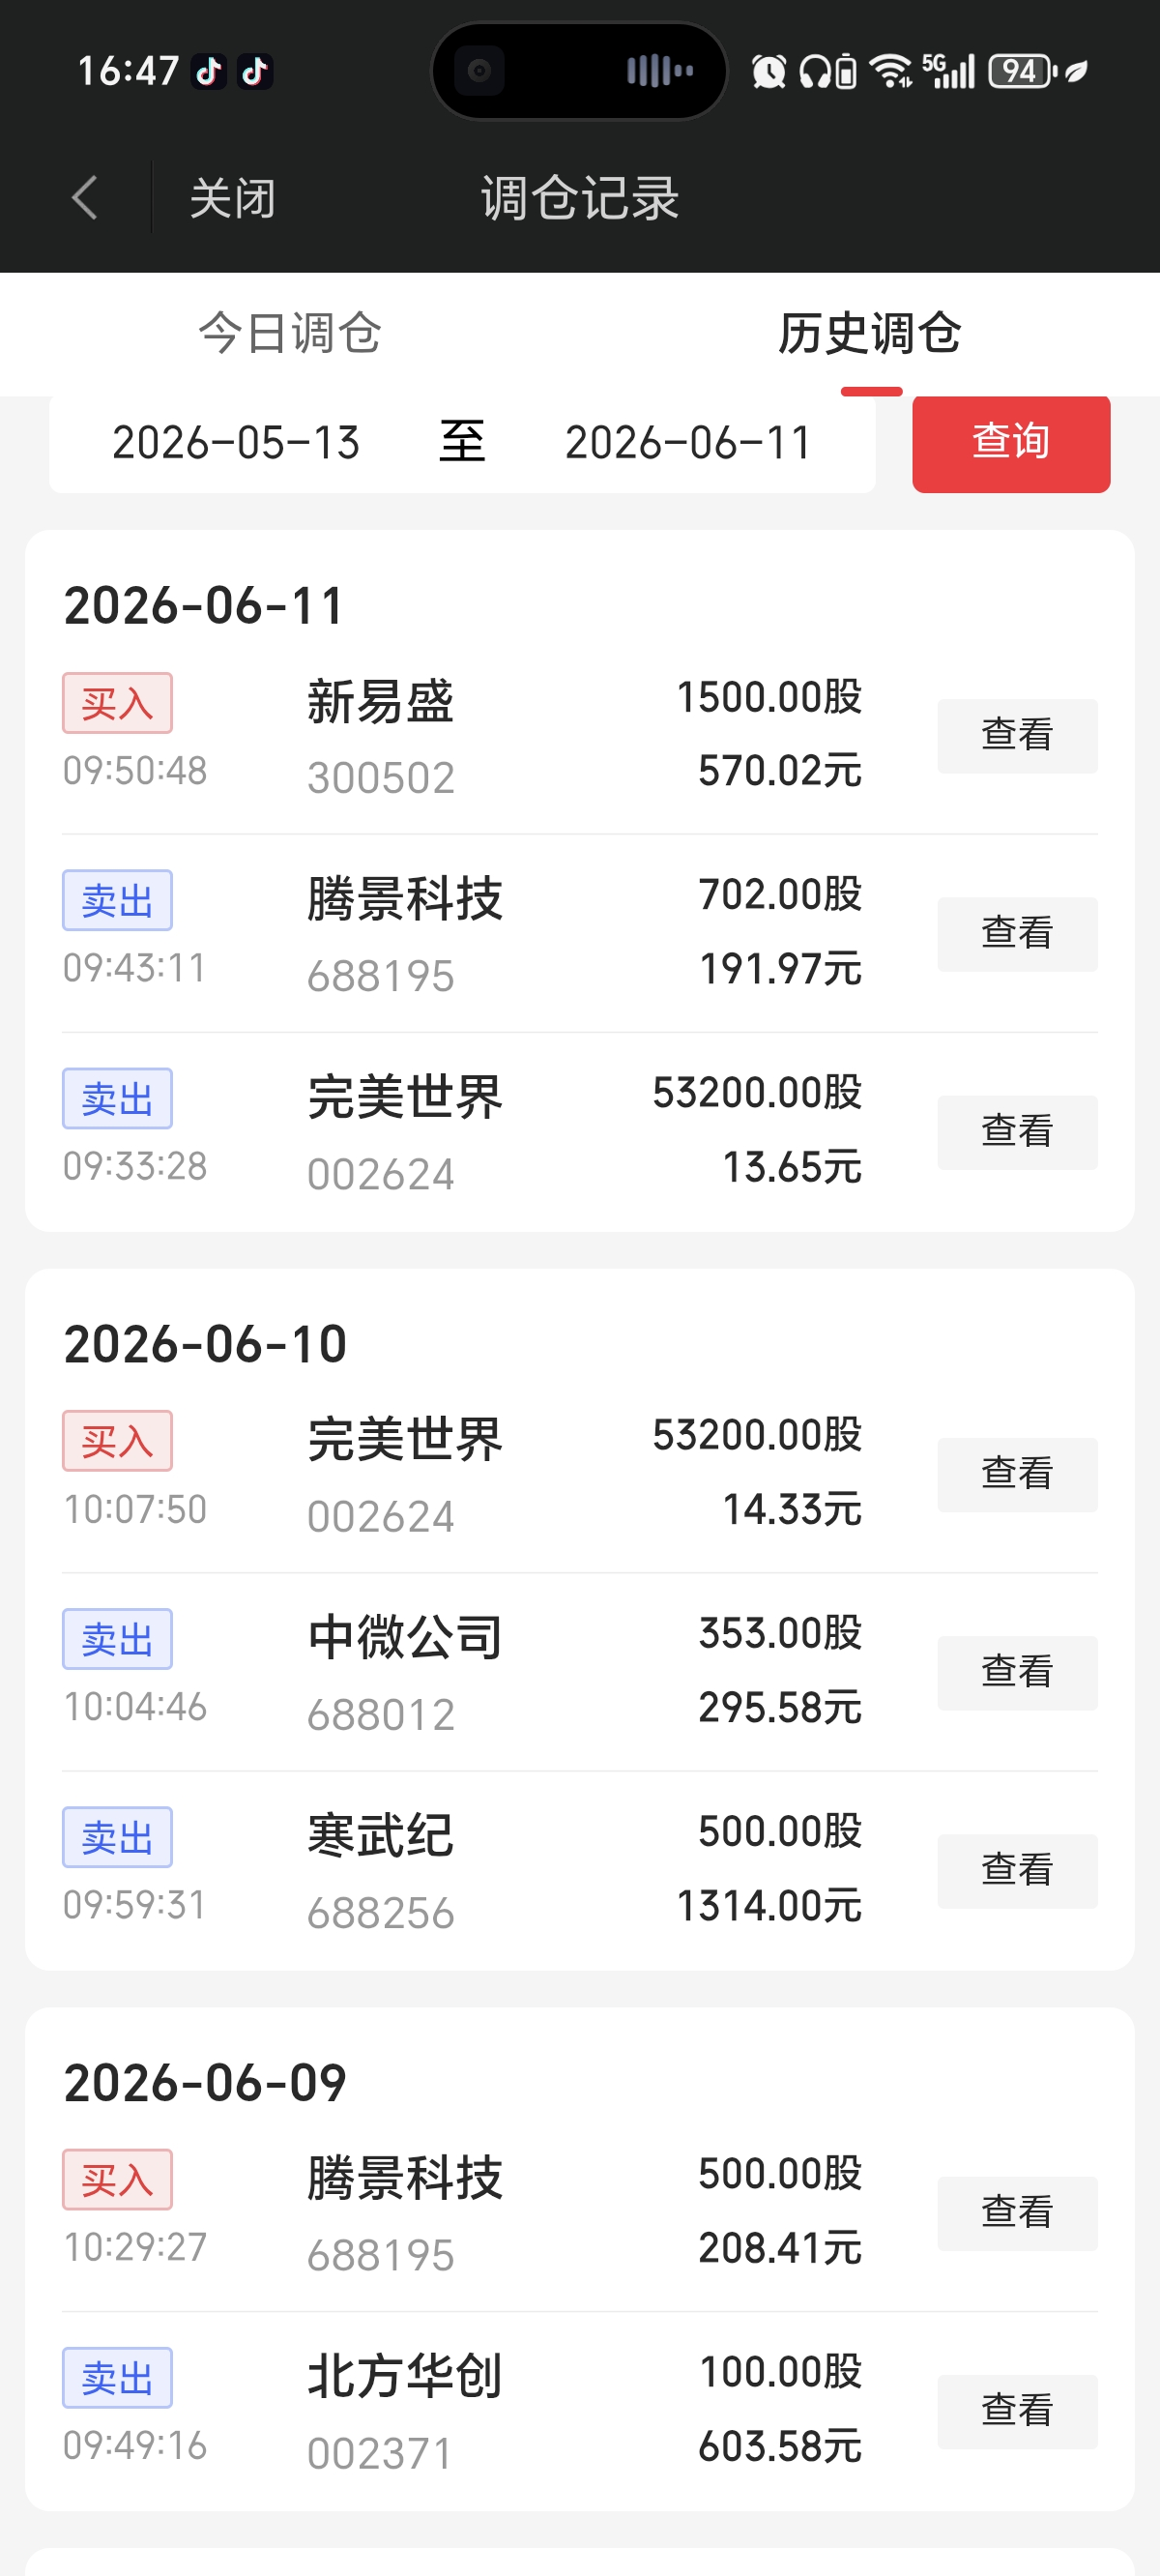
\includegraphics[height=0.30\textheight,keepaspectratio]{pic/Screenshot_20260613_164726_com_hexin_plat_android.jpg}
        \caption{后期调仓记录}
    \end{subfigure}
    \hfill
    \begin{subfigure}{0.43\textwidth}
        \centering
        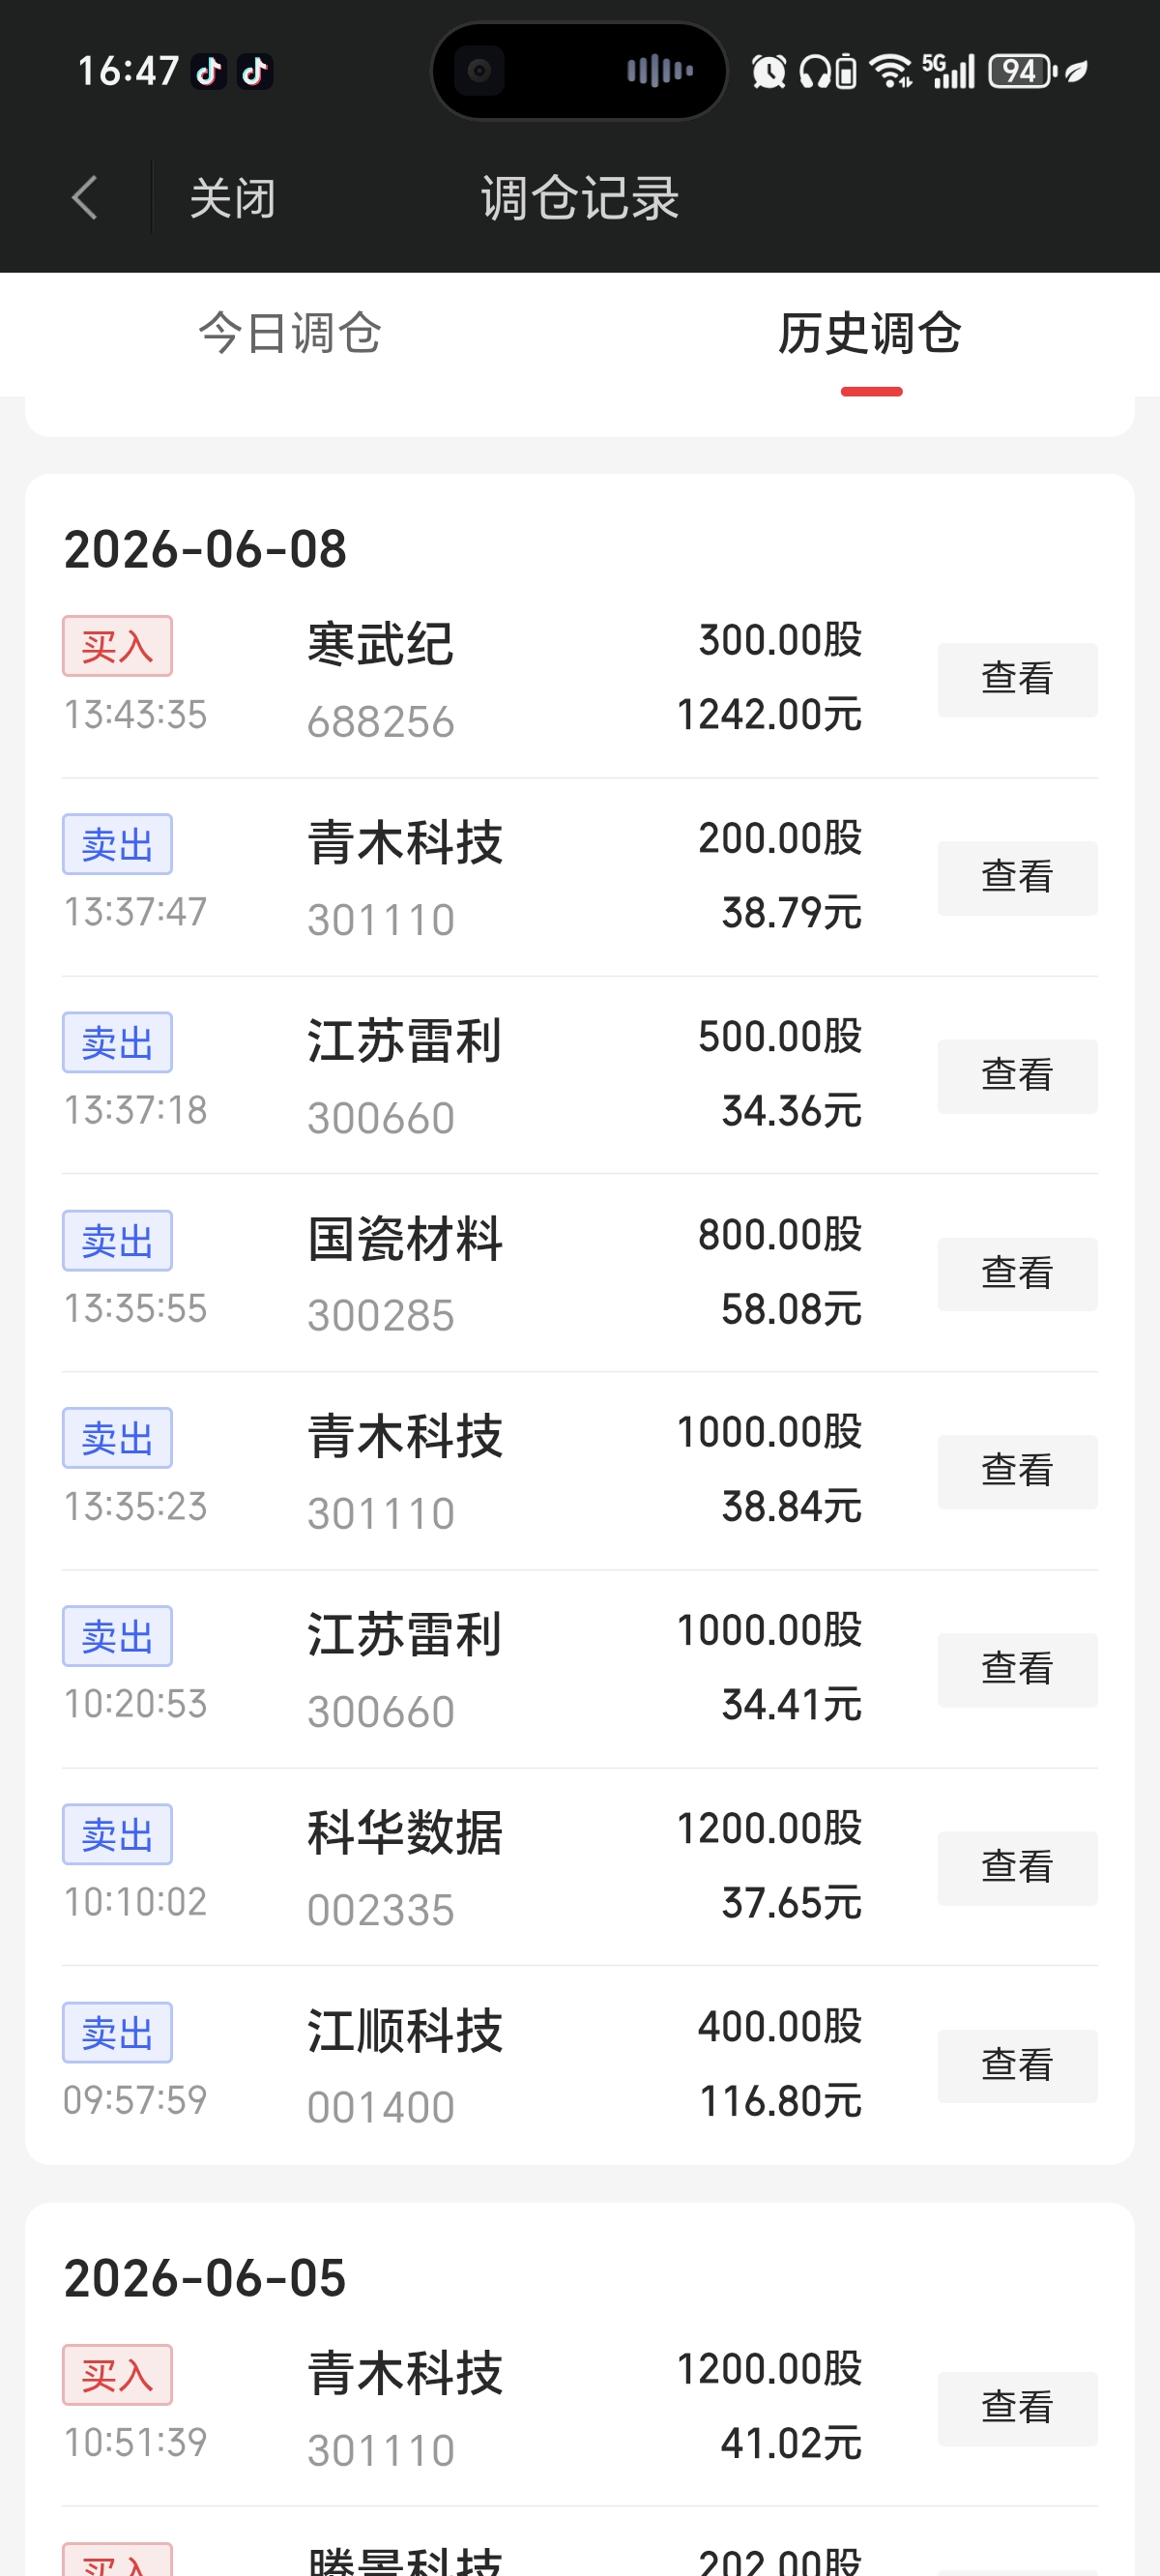
\includegraphics[height=0.30\textheight,keepaspectratio]{pic/Screenshot_20260613_164733_com_hexin_plat_android.jpg}
        \caption{中期调仓记录}
    \end{subfigure}
    \caption{同花顺模拟交易记录示例。完整截图识别结果另存为交易记录整理文件。}
    \label{fig:trading_records}
\end{figure}

\subsection{账户结果}

同花顺模拟交易的最终结果如表~\ref{tab:trading_summary}所示。最终收益为 $-19.40\%$，排名为 $119/119$。这一结果显著弱于离线 holdout 上的模型表现，但它不应被直接解释为 CLIME 排序信号失效。根据交易过程记录，账户在模拟中期仍约为 $-4.82\%$，最终的大幅回撤主要发生在后期少数集中持仓和不利盘中成交之后。因此，本节将该结果视为一个\textbf{执行协议偏离后的异常案例}：它说明日频 alpha 信号若缺少固定调仓协议和自动执行约束，可能被盘中执行误差显著放大。

\begin{table}[H]
    \centering
    \caption{同花顺模拟交易账户结果}
    \label{tab:trading_summary}
    \begin{tabular}{@{}lr@{}}
        \toprule
        指标 & 数值 \\
        \midrule
        总收益率 & $-19.40\%$ \\
        月收益率 & $-19.40\%$ \\
        选股成功率 & $21.90\%$ \\
        最终排行榜名次 & $119/119$ \\
        模拟中期账户收益 & 约 $-4.82\%$ \\
        \bottomrule
    \end{tabular}
\end{table}

\subsection{逐日调仓记录}

表~\ref{tab:daily_rebalance}整理了截图中可识别的逐日调仓记录。可以看到，前期操作更接近分散持仓和日频换仓；后期则逐渐出现更强的人工择时和集中持仓，这也是最终收益被少数交易主导的重要原因。

\begingroup
\footnotesize
\setlength{\tabcolsep}{3pt}
\begin{longtable}{@{}p{0.09\textwidth}p{0.30\textwidth}p{0.30\textwidth}p{0.19\textwidth}@{}}
    \caption{模拟交易逐日调仓记录（根据同花顺截图识别）}
    \label{tab:daily_rebalance}\\
    \toprule
    日期 & 买入 / 加仓 & 卖出 / 减仓 & 执行特征 \\
    \midrule
    \endfirsthead
    \toprule
    日期 & 买入 / 加仓 & 卖出 / 减仓 & 执行特征 \\
    \midrule
    \endhead
    06-01 &
    青龙管业 12.76/12.61，中国银行 5.88，国检集团 7.00，韩建河山 6.06，华电能源 9.69，粤电力A 9.76，阳光股份 4.89，欧晶科技 26.03，新亚电子 25.90 &
    无可见卖出记录 &
    初始建仓，整体较分散，但成交集中在 11:00 后，已不是严格开盘建仓。 \\
    \midrule
    06-02 &
    招商银行 38.83，浙大网新 8.20，红星发展 38.49，胜利精密 3.75 &
    欧晶科技 26.08，中国银行 6.01，华电能源 9.54，韩建河山 6.06，国检集团 7.00，阳光股份 4.93 &
    先释放部分旧仓资金，再买入新组合；整体仍接近日频调仓。 \\
    \midrule
    06-03 &
    光迅科技 227.80，寒武纪 1406.42，裕太微-U 249.00，宝鹰股份 4.76，伊利股份 26.63，中国铁建 6.39，美的集团 82.22，宁德时代 428.00，荣旗科技 83.17，海航控股 1.51，中远海控 14.66 &
    粤电力A 8.65，青龙管业 11.74，招商银行 38.55，红星发展 42.72，浙大网新 7.90，新亚电子 24.50，胜利精密 3.57 &
    大规模换仓；卖出多在早盘完成，买入分布在 10:00 后至下午，存在明显盘中价格路径影响。 \\
    \midrule
    06-04 &
    中微公司 283.99 &
    伊利股份 26.57，光迅科技 223.49，裕太微-U 230.00，宝鹰股份 4.69，美的集团 82.30，海航控股 1.49，中远海控 14.64，中国铁建 6.31 &
    降低前一日持仓，买入集中度开始上升。 \\
    \midrule
    06-05 &
    青木科技 41.02，腾讯科技 246.20，江苏雷利 31.61，江顺科技 110.24，国瓷材料 65.62，北方华创 617.62，寒武纪 1379.99，科华数据 39.04 &
    荣旗科技 83.00，寒武纪 1377.00 &
    当日买入集中在 10:00 后，部分高波动股票盘中买卖，执行误差开始变大。 \\
    \midrule
    06-08 &
    寒武纪 1242.00 &
    青木科技 38.79/38.84，江苏雷利 34.36/34.41，国瓷材料 58.08，科华数据 37.65，江顺科技 116.80 &
    先卖出旧组合再买入新标的；多笔卖出发生在 10:00 后和下午，资金释放与新仓买入存在时滞。 \\
    \midrule
    06-10 &
    完美世界 14.33，腾讯科技 208.41 &
    中微公司 295.58，寒武纪 1314.00，北方华创 603.58 &
    持仓开始明显集中，组合不再严格对应固定 top-$K$ 分散协议。 \\
    \midrule
    06-11 &
    新易盛 570.02 &
    腾讯科技 191.97，完美世界 13.65 &
    后期集中持仓交易；新易盛后续浮亏较大，是最终回撤的重要来源。 \\
    \bottomrule
\end{longtable}
\endgroup

\subsection{盈亏来源分析}

表~\ref{tab:trading_key_trades}列出了若干可配对的代表性盈亏来源。该表只根据截图中的成交价和持仓现价估算，不包含手续费、滑点、印花税和现金占用影响。从结果看，模拟交易并非所有模型相关标的都失败：红星发展、江苏雷利、江顺科技、寒武纪等交易均产生正收益；真正主导最终回撤的是少数后期高波动、集中持仓和不利成交价格。

\begin{table}[H]
    \centering
    \caption{代表性盈亏来源（按截图成交价估算）}
    \label{tab:trading_key_trades}
    \resizebox{\textwidth}{!}{%
    \begin{tabular}{@{}llrrrl@{}}
        \toprule
        股票 & 区间 / 状态 & 买入或成本价 & 卖出或标记价 & 收益率 & 解释 \\
        \midrule
        新易盛 & 最终持仓 & 570.20 & 506.46 & $-11.18\%$ & 后期集中持仓浮亏，是最终回撤的主要来源之一 \\
        完美世界 & 06-10 至 06-11 & 14.33 & 13.65 & $-4.75\%$ & 后期集中交易亏损 \\
        国瓷材料 & 06-05 至 06-08 & 65.62 & 58.08 & $-11.49\%$ & 买入后出现较大回撤 \\
        粤电力A & 06-01 至 06-03 & 9.76 & 8.65 & $-11.37\%$ & 前期大额亏损来源 \\
        青木科技 & 06-05 至 06-08 & 41.02 & 38.83 & $-5.33\%$ & 执行路径不利 \\
        红星发展 & 06-02 至 06-03 & 38.49 & 42.72 & $+10.99\%$ & 明显盈利交易 \\
        江苏雷利 & 06-05 至 06-08 & 31.61 & 34.39 & $+8.79\%$ & 明显盈利交易 \\
        江顺科技 & 06-05 至 06-08 & 110.24 & 116.80 & $+5.95\%$ & 盈利交易 \\
        寒武纪 & 06-08 至 06-10 & 1242.00 & 1314.00 & $+5.80\%$ & 高波动标的中的盈利交易 \\
        \bottomrule
    \end{tabular}%
    }
\end{table}

\subsection{执行偏差与结果解释}

本次模拟交易最重要的经验是：\textbf{模型预测任务、组合选择任务和交易执行任务不能混为一谈}。CLIME 在训练和验证阶段优化的是下一交易日的横截面收益排序；也就是说，它回答的问题是：在给定第 $t$ 日以前的信息后，哪些股票在第 $t+1$ 日更可能排在收益靠前的位置。这个任务天然适合用 RankIC、top-$K$ 收益、分组收益等指标评价，但它并不直接回答盘中买点、卖点、成交价、资金释放顺序、换手成本、仓位集中度和人工执行纪律等问题。因此，模拟交易中的最终收益并不是模型分数的单一函数，而是多个模块共同作用后的结果。

为了更清楚地区分这些因素，可以将真实模拟收益理解为如下几类影响的叠加：
\begin{equation}
    R_{\mathrm{realized}}
    =
    R_{\mathrm{alpha}}
    +
    R_{\mathrm{portfolio}}
    +
    R_{\mathrm{execution}}
    +
    R_{\mathrm{discretion}},
\end{equation}
其中 $R_{\mathrm{alpha}}$ 来自 CLIME 对股票相对收益强弱的排序能力，$R_{\mathrm{portfolio}}$ 来自 scorer 和 selector 如何把排序分数转化为持仓组合，$R_{\mathrm{execution}}$ 来自具体成交时点、成交价格和资金约束，$R_{\mathrm{discretion}}$ 则来自手动执行中的临时判断和策略一致性偏移。离线实验主要隔离评估 $R_{\mathrm{alpha}}$，而同花顺模拟交易同时混入了后面三项。因此，当模拟交易出现 $-19.40\%$ 时，更合理的解释不是“CLIME 没有学到 alpha”，而是“alpha 信号在未被严格执行协议保护的情况下，被组合构造和盘中执行误差显著稀释甚至反转”。

表~\ref{tab:execution_gap_framework}进一步总结了本次模拟交易中的主要偏差来源。可以看到，最终收益较差并不是由单一原因造成的，而是多个现实交易约束共同叠加后的结果。尤其是对于一个日频 ranking 模型而言，只要执行价格不再接近统一调仓价格，离线排序优势就可能被日内价格路径显著削弱。

\begin{table}[H]
    \centering
    \caption{模拟交易结果的执行偏差归因框架}
    \label{tab:execution_gap_framework}
    \footnotesize
    \begin{tabular}{@{}p{0.18\textwidth}p{0.27\textwidth}p{0.25\textwidth}p{0.22\textwidth}@{}}
        \toprule
        偏差来源 & 具体表现 & 对结果的影响 & 对模型评价的含义 \\
        \midrule
        日频预测与盘中执行不一致 &
        模型预测下一交易日收益排序，但实际买入常发生在 10:00 后或下午 &
        若标的早盘已上涨，实际买入价会消耗原本的日频 alpha &
        该误差主要属于执行层，而不是预测器本身 \\
        \midrule
        先卖后买的资金释放约束 &
        需要先卖出旧仓才能买入新推荐股票，旧仓低开时容易延迟换仓 &
        等待旧仓反弹会错过新仓更优价格，形成路径依赖 &
        离线 top-$K$ 评估默认同步调仓，未覆盖该约束 \\
        \midrule
        弱势市场中的人工择时压力 &
        连续下跌时更容易等待反弹、推迟卖出或临时改变买入节奏 &
        执行逐渐偏离固定、机械、可复现的交易协议 &
        该部分属于人工决策项，会污染模型信号评价 \\
        \midrule
        后期仓位集中 &
        后期少数股票持仓权重明显上升，例如新易盛、完美世界 &
        个股波动被放大，最终收益被少数交易主导 &
        结果不再等价于分散 top-$K$ 排序策略 \\
        \midrule
        缺少自动化执行模块 &
        没有固定开盘执行、成交价控制、滑点建模和仓位上限 &
        真实收益同时混入成交价格、人工判断和市场路径 &
        暴露的是完整交易系统缺口，而非单纯阿尔法模型缺口 \\
        \bottomrule
    \end{tabular}
\end{table}

第一层偏差来自\textbf{预测标签与成交价格之间的时间尺度不一致}。CLIME 的标签是下一交易日收益排序，本质上接近一个日频 close-to-next-day 的相对比较问题；但模拟交易中的盈亏由真实成交价决定。如果模型在前一晚给出某只股票的高分，理想执行应当在固定调仓时点迅速买入，至少要保证不同股票之间的执行价格具有可比性。但实际操作中，许多买入并没有发生在 9:30 附近，而是发生在 10:00 之后甚至下午。对于日内波动较大的股票，如果其早盘已经上涨，那么晚买入会显著抬高成本，原本属于模型预测的日频 alpha 会被盘中价格变化吃掉。反过来，如果股票高开低走，模型可能在日频收益上仍然判断正确，但由于买在盘中高位，真实账户仍会亏损。也就是说，CLIME 预测的是“哪只股票下一天更值得买”，而模拟交易还额外要求回答“以什么价格买到它”，后者并不在模型训练目标之内。

第二层偏差来自\textbf{先卖后买的资金释放约束}。离线回测通常默认可以在统一调仓时点将旧组合切换到新组合，或者至少默认卖出和买入可以近似同步完成。但在真实模拟账户中，买入新推荐股票之前往往必须先卖出旧持仓释放资金。弱势市场会显著放大这个约束：旧持仓低开时，立即卖出会锁定亏损；等待旧持仓反弹，则可能错过新推荐股票的早盘买点。这就形成了一个路径依赖问题：为了避免在旧仓低点卖出，执行会被迫延后；而一旦执行延后，原本想买入的新股票可能已经上涨，导致买入价格恶化。前面调仓表中多笔买入分布在 10:00 后和下午，正说明最终收益已经不只是模型排序结果，而是被“旧仓卖出时点”和“新仓买入时点”共同决定。

第三层偏差来自\textbf{弱势市场下的人工执行压力}。从交易过程看，模拟期间整体市场环境并不友好，连续下跌会使执行者面临更强的心理压力：一方面，旧仓下跌时不愿在低位卖出；另一方面，新推荐股票若早盘上涨，又容易出现追高买入或放弃买入之间的摇摆。于是，交易行为会逐渐偏离一个固定、机械、可复现的量化协议，转而混入等待反弹、人工择时、风险厌恶和短期情绪等因素。这一点也解释了为什么账户中期仍约为 $-4.82\%$，但后期快速扩大到 $-19.40\%$：最终回撤并不是平滑地来自所有交易，而是在市场压力下被少数高波动交易和不利成交路径集中放大。

第四层偏差来自\textbf{仓位集中度与策略一致性偏移}。离线 ranking 评估通常使用 top-$K$ 分散组合来检验排序信号，核心思想是用一组高分股票的平均表现抵消个股噪声。但后期模拟交易逐渐转向少数股票的集中持仓，例如新易盛、完美世界等交易对最终账户收益产生了过高影响。这种集中持仓会把 ranking 模型的横截面优势转化为个股短期波动暴露：如果集中标的方向正确，收益可能迅速改善；但如果买入时点不利或个股当天波动反向，亏损也会被快速放大。表~\ref{tab:trading_key_trades}中，红星发展、江苏雷利、江顺科技、寒武纪等交易仍然产生正收益，说明并不是所有模型相关交易都失败；真正主导最终回撤的是新易盛、完美世界、国瓷材料、粤电力A等少数亏损较大的交易。这说明最终结果更接近“执行层和仓位层对收益分布的重加权”，而不是纯粹的 alpha 排序失败。

第五层偏差来自\textbf{模拟交易协议与离线验证协议不完全一致}。离线验证阶段的核心是可复现：固定样本、固定标签、固定 top-$K$ 规则、固定评价指标，因此不同模型之间可以横向比较。而模拟交易阶段如果没有严格规定“每天何时卖出、何时买入、是否等权、最大单票仓位、是否允许人工覆盖模型推荐、是否允许后期集中持仓”等细节，那么最终结果就会同时反映模型、策略、人工判断和市场运气。这个问题在真实量化系统中通常由 execution engine 和 portfolio optimizer 解决，而不是由 predictor 本身解决。因此，本次交易模拟更像是一次端到端系统压力测试：它暴露的是从研究型 alpha 模型走向可交易系统时，哪些工程约束还没有被完全固定。

在这个意义上，$-19.40\%$ 可以被解释为一个\textbf{执行协议偏离后的异常结果}，而不是 CLIME 离线排序能力的正常外推。更准确地说，它说明：如果没有固定调仓时点、自动化执行、仓位上限、换手约束、交易成本建模、T+1 约束处理、盘中成交价格控制和风险暴露管理，那么即使离线模型具有较好的横截面排序能力，最终模拟收益也可能被人工执行误差、市场路径和集中持仓显著削弱。该结果本身虽然非常差，但它是一个有价值的 failure case，因为它把离线预测和真实交易之间缺失的中间层清楚暴露出来。

这也反过来支持了本文前面对系统架构的拆分：predictor 负责输出可排序的 alpha 信号；risk predictor 负责估计历史波动和下行风险；scorer 负责根据收益偏好和风险偏好生成最终分数；selector 负责构造组合；execution 则负责把组合以固定、可复现、低滑点的方式落地。本次模拟交易中，问题最明显地出现在 selector 之后的 execution 层，而不是 predictor 本身。因此，本文没有把模拟交易结果作为 CLIME 模型能力的主要评价指标，而是将其作为对完整量化交易系统的反思：一个 solid 的预测模型只是系统的一部分，只有当交易协议也被形式化之后，离线 ranking 优势才可能稳定转化为真实收益。

\subsection{小结}

同花顺模拟交易给出的结论是：日频 alpha 模型本身并不等价于完整量化交易系统。CLIME 可以提供横截面排序信号，但若要稳定转化为真实收益，还需要独立的 portfolio construction 和 execution 模块，包括固定调仓时间、仓位上限、换手约束、交易成本建模、自动化下单和盘中成交价格控制。本次 $-19.40\%$ 的结果虽然非常差，但它的价值在于暴露了离线模型到真实交易之间的执行层缺口，也进一步说明本文将“预测排序”和“交易执行”拆分讨论是必要的。

\clearpage
